

\begin{enumerate}
	\item {The note heard on a musical string instrument (e.g. a guitar, violin, etc...) is related to its fundamental frequency. A guitarist tunes their instrument by turning pegs on the bridge causing the tension in the string to increase or decrease. If a guitarist notices that a certain string is sounding “flat” (meaning it is playing a note with a lower frequency than desired), should she tighten or loosen the string ?}
	\begin{enumerate}
		\item[\textbf{Answer: }] {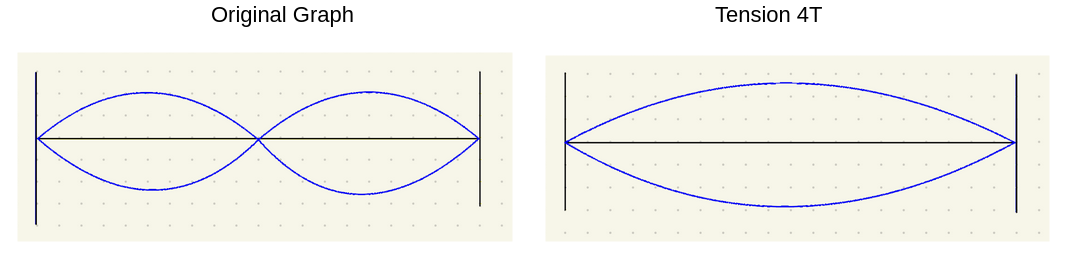
\includegraphics[width=15cm]{Disscussion_1_2302.png}}
	\end{enumerate}
	\item {Suppose that for a particular setup, the hanging mass is 200g, and the $n = 3$ mode is found to have a driving frequency of 80Hz. If the mass is changed to 300g, what frequency will lead to the $n = 4$ mode with this heavier mass?}
	\begin{enumerate}
		\item[\textbf{Answer: }] {This specific set up uses 2 different nodes, 2 different masses and a frequency and is required to find the second frequency, $m_{1} = 0.25kg$, $n_{1} = 3$, $f_{1} = 80Hz$ \& $m{2} = 0.3kg$, $n_{2} = 4$, $f_{2} = ?$. We have, $$\mu_{1} = \mu_{2}$$ $$\frac{m_{1}n_{1}^2}{4f_{1}L^2} = \frac{m_{2}gn_{2}^2}{4f_{2}l^2}$$ $$f_{2} = \sqrt{m_{2}n_{2}^2\frac{f_{1}^2}{m_{1}n_{1}}} \approx 131\text{ Hz}$$}
	\end{enumerate}
	\item {Suppose that instead of both ends being fixed, the end of the string at $x = L$ is free to move up and down. Then, the point at $x = L$ is an antinode and not a node. Start with the equation for a standing wave $y_{standing}(x, t) = 2A\sin(kx)\cos(ωt)$ and derive the condition for the resonant frequencies $f_{n}$ in terms of $n$, $v$ and $L$ ?}
	\begin{enumerate}
		\item[\textbf{Answer: }] {Equation used for standing waves on a string is $y(x, t) = 2A\sin(kx)\cos(\omega t)$ (where $k$ represents the wave number, \textit{A} represents amplitude, $\omega$ represents angular frequency, \textit{x} represents position and \textit{t} represents time.). Due to $x=L$ being an anode, these conditions show, $y(0, t) = 0$ \& $y^{\prime}(L, t) = 0$. Also as $k = n\pi/L$, $\omega = vk$ \& $\omega = vn\pi/L$, we have, Resonance frequency of $f_{n} = vxn/2L$}
	\end{enumerate}
\end{enumerate}

